\chapter{Distributed Coordination}
\section{Election Algorithms}
Distributed algorithms often elect one process to act as a coordinator or a server. We assume each process is assigned a unique process number, that a process knows all process numbers, and a process does not know which process numbers are alive.

The election process proceeds as follows: \begin{itemize}
\item Select the maximum process number among active processes.
\item Appoint the process the coordinator.  
\item All the processes must agree upon this decision. 
\end{itemize}

\subsection{Bully Algorithm (Garcia-Molina)}
When a process $P$ notices that the coordinator is no longer responding to requests, it initiates an election. 

$P$ sends an \textit{Election} message to all processes with higher numbers. If one of the higher numbered answers, that process becomes the new leader. If no one responds, $P$ wins the election and becomes coordinator. Note that timeout overhead and delayed responses are a consideration.

At any moment, a process can get an \textit{Election} message from one of its lower-numbered colleagues. The receiver sends an \textit{OK} message back to the sender. The receiver then holds an election, unless it is already holding one. 

Eventually, all processes give up but one, and that one is the new coordinator. It announces its victory by sending \textit{Coordinator} messages to all processes. If a process that was previously down comes back up, it holds an election. If it happens to be the highest-numbered process currently running, it will win the election and take over the coordinator's job.  The highest numbered process always wins, hence the name "bully algorithm." 

\subsection{Ring Algorithm}
Processes form a logical ring. Each process knows which process comes after it. If a process finds the coordinator dead, it sends an \textit{Election} message which contains its own process number to its successor in the ring. If the successor is down, the message is sent to the next process along the ring. 

When receiving an \textit{Election} message, each process appends its process number to the message and then forwards it to the successor. When the message returns to the process that originally sent the message, the process changes the message type from a \textit{Election} message to a \textit{Coordinator} message and circulates the message again. 

The purpose of the \textit{Coordinator} message is to inform all processes that the highest-numbered process is the new coordinator and the processes contained in the message are the members of the ring. 

\section{Distributed Transactions}
\subsection{Atomic Transactions}
An atomic transaction provides a view where either a set of operations have all been completed or none of them have been completed.

First, a process declares to all other processes (involved in a transaction) that it is starting the transaction. The processes exchange information and perform their specific operations. The initiator announces that it wants all the other processes to \textit{commit} to all the operations done up to that point. 

If all processes agree to commit, the results are made permanent. If at least one of the processes refuse, all the states - usually opened files/databases (on all machines) - are reverted to the point prior to starting the transaction. 

A set of assumptions must be made when working with distributed transactions. These are: \begin{itemize}
\item A system consists of independent processes where each process may fail at random.
\item No communication errors may be encountered.  
\item \textit{Stable storage} is available; this guarantees no data is lost unless the storage is physically lost by disasters such as floods or earthquakes. 

\textit{Note}: Data in RAM disappears when the power is turned off. Data in a disk becomes inaccessible if the head crashes. As a result, these are not stable storage.
\end{itemize}

Stable storage can be implemented with a pair of disks, as seen in \autoref{fig:screenshot045}. Each block on drive 2 is a copy of the corresponding block on drive 1. When a block is updated, the block on drive 1 is first updated and verified. Then, the same block on drive 2 is updated and verified. 

\begin{figure}
\centering
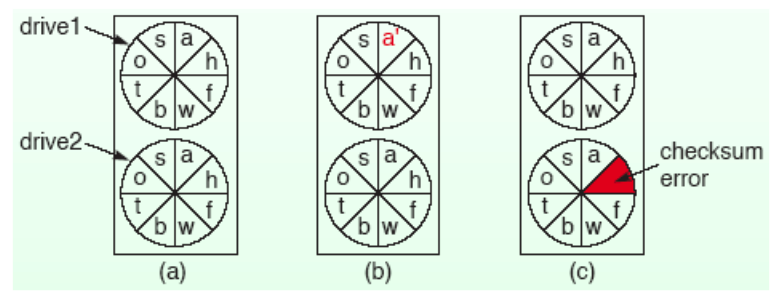
\includegraphics[width=0.7\linewidth]{screenshot045}
\caption{Stable storage using a pair of disks.}
\label{fig:screenshot045}
\end{figure}

If the system crashes after the update of drive 1 but before the update of drive 2, the blocks on the two drives are compared and the blocks on drive 1 are copied to drive 2 after system reboot. If a checksum error is encountered because of a bad block, the block is copied from the disk without an error. 

\subsection{Primitives}
Programming a transaction requires special primitives that must be supplied by the OS or by the programming language. These primitives are implemented as either system calls, library functions, or constructs of a programming language.  Examples of the primitives include: \begin{itemize}
\item \textbf{Begin Transaction}: Specifies the beginning of a transaction. 
\item \textbf{End Transaction}: Specifies the end of a transaction, and tries to commit the results. 
\item \textbf{Abort Transaction}: Abort the transaction and restore the old state.
\item \textbf{Read}: Reads data from a file. 
\item \textbf{Write}: Writes data to a file. 
\end{itemize}

Begin Transaction and End Transaction specify the scope of a transaction. The operations delimited by the two operations form the transaction. 

\subsection{Properties}
Any transaction must abide by these four essential properties: \begin{itemize}
\item \textbf{Atomicity}: A transaction happens indivisibly to the outside world. (Either all operations of the transaction are completed or none are completed.) The other process cannot observe the intermediate states of the transaction. 

\item \textbf{Consistency}: A transaction does not violate system invariants. For example, an invariant in a banking system may be the law of conversation regarding the total amount of money - that is, the sum of money in the source and destination accounts after any transfer is the same as the sum before the transfer (although conservation may be violated during the transfer). 

\item \textbf{Isolation}: Even if more than one transaction is running simultaneously, the final result is the same as the result of running the transactions sequentially in some order. This property is also called \textit{serializable}.

\item \textbf{Durability}: Once a transaction commits, changes are permanent. No failure after the commit can undo the results or cause these to be lost. 
\end{itemize}

\subsection{Nested Transactions}
Transactions may contain their own sub-transactions; these are referred to as \textit{nested transactions}. They are subject to a potential problem: \begin{itemize}
\item Assume a transaction starts several sub-transactions in parallel.  
\item One of these sub-transactions commits and makes its results visible to the parent transaction. 
\item For some reason, the parent transaction is aborted and the entire system needs to be restored to its original state. 
\item Consequently, the results of the sub-transaction that committed must be undone. 
\item Undo-ing a committed transaction is a violation of transaction laws.
\end{itemize}

To alleviate this, we define characteristics for the nested transactions: \begin{itemize}
\item Permanence of a sub-transaction is only valid within the world of its direct parent and is otherwise invalid/irrelevant in the context of further ancestors.
\item Permanence of a transaction is only valid for the outermost transaction (that is, the top-level transaction that is itself not nested in another transaction).
\end{itemize}

To facilitate this, one method is to have each sub-transaction make a private copy of all objects in the system. If a sub-transaction commits, its private copy of the mutated resources replaces its parent's copy. This limits any potential mutation to the scope of the parent transaction, so that the outside world is not affected until the parent transaction commits.

\subsection{Implementation of atomic transactions}
Implementing atomic transactions involves the hiding of operations within a transaction from outer processes, making the results visible only after commit and restoring the old state if the transaction is aborted.

There are two ways to restore the old state: \textit{private workspaces}, and \textit{write-ahead logs}. These are discussed in more detail below.

\subsubsection{Private Workspace}
When a process starts a transaction, it is given a private workspace containing all the objects including data and files. Read and write operations are performed within the private workspace. The data within the private workspace is written back when the transaction commits. 

The problem with this technique is that the cost of copying every object to a private workspace is high. The following optimisation is possible: if a process only reads an object, there is no need for a private copy; if a process updates an object, a copy of the object is made in the private workspace. 

If we use indices to objects, we can reduce the number of copy operations. When an object is to be updated, a copy of the index of each object is made in the private workspace. When an object is mutated, its private index is updated. On commit, the private index is copied to the parent's index. This is illustrated in \autoref{fig:screenshot046}.

\begin{figure}
\centering
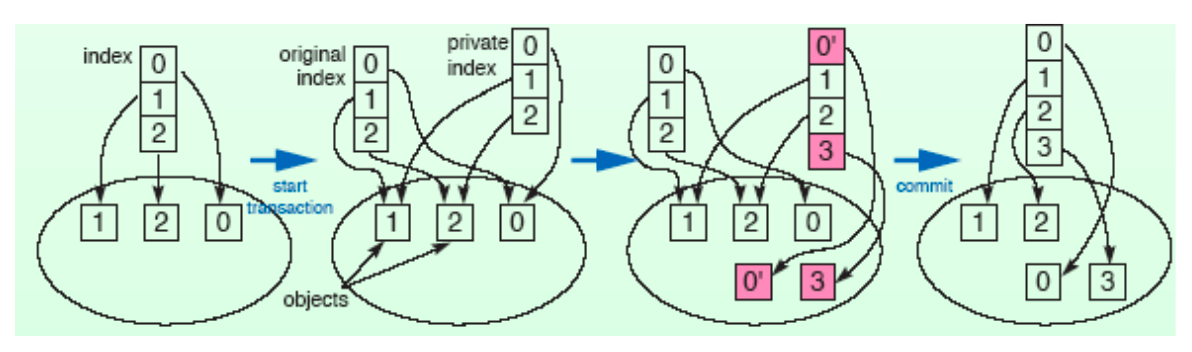
\includegraphics[width=0.7\linewidth]{screenshot046}
\caption{Optimising the private workspace technique using indices.}
\label{fig:screenshot046}
\end{figure}

If the transaction aborts, the private copies of the objects and indices are discarded, as shown in \autoref{fig:screenshot047}.
\begin{figure}
\centering
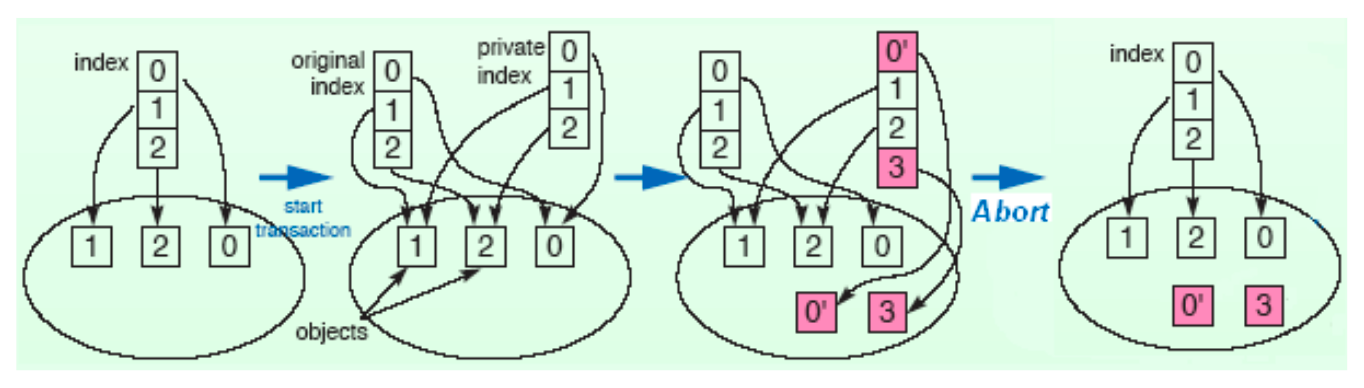
\includegraphics[width=0.7\linewidth]{screenshot047}
\caption{Aborted optimised private workspace tranction.}
\label{fig:screenshot047}
\end{figure}

\subsubsection{Write-ahead Log} 
Before any changes to objects are made, a record is written to a \textit{write-ahead log} on stable storage. The log contains the following information: which transaction is making the change, which object is being changed, and what the old and new values are. 

The change is made to the object only after the log has been written successfully. If the transaction committed, a commit record is written to the log (data has already been written). If the transaction aborts, the log can be used to rollback to the original state. The log can be used for recovering from crashes. 

\subsubsection{Two-Phase Commit Protocol}
The action of committing a transaction must be done instantaneously and indivisibly. In a distributed system, the commit requires the cooperation of multiple processes that may be on different machines. Two-phase commit protocol is the most widely used protocol to implement an atomic commit. 

One process functions as the coordinator. The other participating processes are subordinates (Cohorts). This is shown in \autoref{fig:screenshot048}.

\begin{figure}
\centering
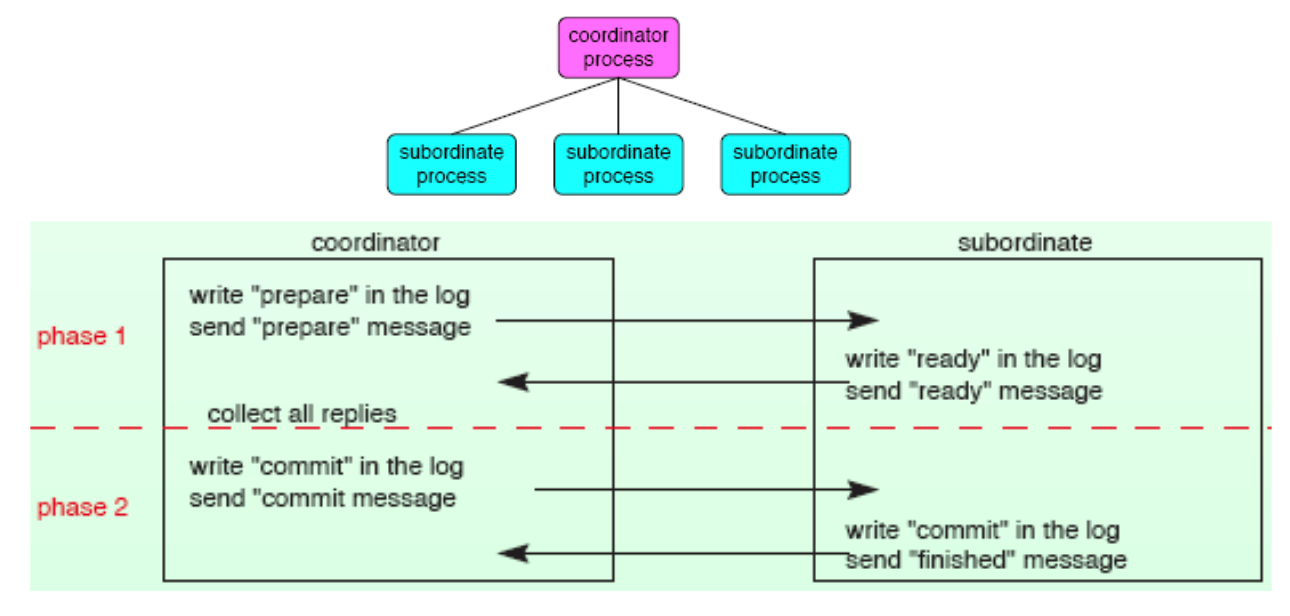
\includegraphics[width=0.7\linewidth]{screenshot048}
\caption{Two-phase commit protocol.}
\label{fig:screenshot048}
\end{figure}

The coordinator writes an entry \textit{prepare} in the log on stable storage and sends the other processes involved (the subordinates) a message telling them to prepare. When a subordinate receives the message, it checks to see if it is ready to commit, makes a log entry, and sends back its decision. 

After collecting all the responses, if all the processes are ready to commit, the transaction is committed. Otherwise, the transaction is aborted. The coordinator writes a log entry and then sends a message to each subordinate informing it of the decision. The action of the coordinator writing the commit to the log is equivalent to committing the transaction; no rolling back can occur afterwards, regardless of what may happen.

This protocol is highly resilient in the face of crashes because it uses stable storage. If the coordinator crashes after writing a \textit{prepare} or \textit{commit} message, it can still resume from its previous state.

If a subordinate crashes after writing a \textit{ready} or \textit{commit} log entry, it can resume from a \textit{ready} or \textit{finished} message upon restarting.

\subsubsection{Three-Phase Commit Protocol}
This protocol assumes that each site uses the write-ahead log protocol, and that at most one site can fail during the execution of the transaction.

Before the commit protocol begins, all the sites are in state $q$. If the coordinator fails while in state $q1$, all the cohorts perform the \textit{timeout transition}, thus aborting the transition. Upon recovery, the coordinator performs the \textit{failure transition}. \footnote{No, I'm not entirely sure what this protocol is or what it has to offer, either.}

\section{Concurrency Control}
When several transactions run simultaneously in different processes, we must guarantee the final result is the same as the result of running the 
transactions sequentially in some order. That is, we need a mechanism to guarantee isolation or serializability. This mechanism is \textit{concurrency control}. 

There are three typical algorithms: using locks, using timestamps, and being optimistic.

\subsection{Locks}
This is the oldest and most widely used concurrency control algorithm. When a process needs to access shared resource as part of a transaction, it first locks the resource. If the resource is locked by another process, the requesting process waits until the lock is released. 

The basic scheme is overly restrictive. The algorithm can be improved by distinguishing read locks from write locks. Data that only needs to be read (referenced) is locked in shared mode. Data that needs to be updated (modified) is locked in exclusive mode. 

Lock modes have the following compatibility: \begin{itemize}
\item If a resource is not locked or locked in shared mode, a transaction can lock the resource in shared mode. 
\item A transaction can lock a resource in exclusive mode only if the resource is not locked. 
\end{itemize}
This is shown in \autoref{tab:lockmodes}.

\begin{table}
\caption{Compatibility between lock modes.}
\label{tab:lockmodes}
\centering
\begin{tabular}{|c|c|c|c|}
\hline
& \multicolumn{3}{|c|}{\textbf{Locking Mode}} \\
\hline
\textbf{Locking Mode} & Unlocked & Shared & Exclusive \\
\hline
Shared & \cmark & \cmark & \xmark \\
\hline
Exclusive & \cmark & \xmark & \xmark \\
\hline
\end{tabular}
\end{table}

If two transactions are trying to lock the same resource in incompatible modes, the two transactions are in \textit{conflict}. A conflict relationship can be a shared-exclusive conflict (or read-write conflict) or a exclusive-exclusive conflict (or write-write conflict).

\subsubsection{Two-Phase Locking}
Using locks does not necessarily guarantee serializability. Only transactions executed concurrently in accordance with the following steps will be serializable: \begin{enumerate}
\item A transaction locks a shared resource before accessing the resource and releases the lock after using it.
\item Locking is granted according to the compatibility constraint.
\item A transaction does not acquire any locks after releasing a lock.
\end{enumerate}
The use of locks in a manner that satisfies the above conditions is referred to as the \textit{two-phase locking protocol}.

A transaction acquires all necessary locks in the first phase; the \textit{growing phase}. The transaction releases all the locks in the second phase; the \textit{shrinking phase}. Two-phase locking is sufficient to guarantee serializability.

Suppose a transaction aborts after releasing some of the locks. If other transactions have used resources protected by these released locks, these transactions must also be aborted; this is referred to as a \textit{cascading abort}, as seen in \autoref{fig:screenshot049}.

\begin{figure}
\centering
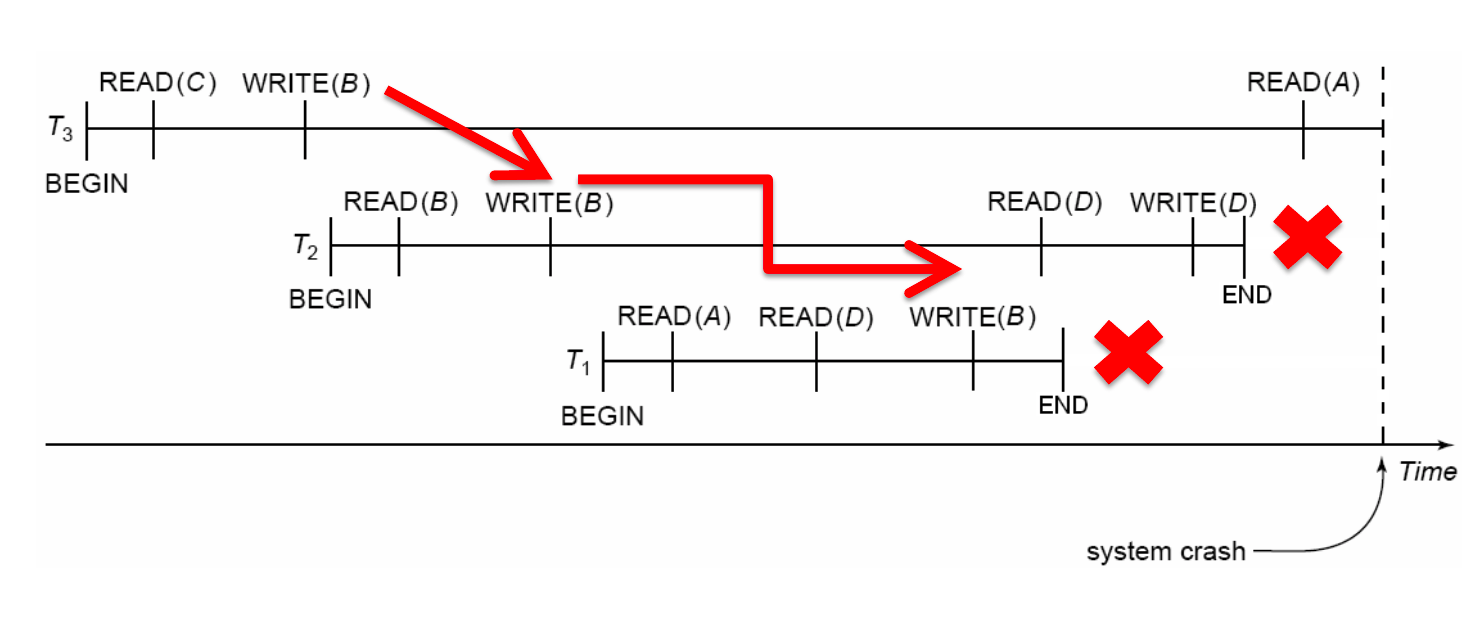
\includegraphics[width=0.7\linewidth]{screenshot049}
\caption{Cascading abort in two-phase locking.}
\label{fig:screenshot049}
\end{figure}

To avoid cascading abort, many systems use \textit{strict two-phase locking} in which transactions do not release any locks until the transaction is fully committed. The sequence for strict two-phase locking follows: \begin{enumerate}
\item Begin transaction
\item Acquire locks before reading or writing resources
\item Commit changes
\item Release all locks
\item End transaction
\end{enumerate}

Strict two-phase locking has the following advantages: \begin{itemize}
\item A transaction always reads a value written by a committed transaction. A transaction never has to be aborted - the cascading abort never happens. 
\item All lock acquisitions and releases can be handled by the system without the transaction being aware. Locks are acquired whenever data is accessed and released when the transaction has finished. 
\end{itemize}

However, two-phase locking can cause deadlocks to occur. This will happen when two processes try to acquire the same pair of locks but in reverse order to each other.

\subsubsection{Granularity}
The \textit{lock granularity} refers to the size of resources that can be locked by a single lock. Finer granularity allows for more concurrent processing, but requires a greater quantity of locks.

For example, consider locking by file and locking by record contained in a file. Suppose that two transactions access different records in the same file. If the record is the unit of lock, two transactions can access the data simultaneously. On the other hand, if the file is the unit of lock, the two transactions cannot access the data simultaneously. 

\subsection{Timestamps}
Assign each transaction a timestamp when the transaction begins. These timestamps must be unique; this can be ensured using 
Lamport's algorithm. 

Each resource has a \textit{read timestamp} and a \textit{write timestamp}. A read timestamp is the timestamp of the transaction which read the resource most recently. A write timestamp is the timestamp of the transaction which updated the resource most recently. However, note that read timestamps and write timestamps are \textit{not} the actual time values for when the data items were read or written.

Let $\mathtt{TRD}(x)$ be the read timestamp of resource $x$.  Let $\mathtt{TWR}(x)$ be the write timestamp of resource $x$. 

When a transaction with timestamp $T$ tries to read resource $x$, \begin{itemize}
\item $T < \mathtt{TWR}(x)$ implies that the transaction is attempting to read a $x$ that has already been overwritten. As a result, the request is rejected and the transaction is aborted.
\item $T \ge \mathtt{TWR}(x)$ implies that the transaction is attempting to read a value after its last write, so the transaction is allowed to read the resource. 
\end{itemize}

When a transaction with timestamp $T$ tries to update resource $x$, \begin{itemize}
\item $T < \mathtt{TWR}(x)$ implies that the transaction is attempting to write an old $x$. As a result, the request is rejected and the transaction is aborted.
\item $T < \mathtt{TRD}(x)$ implies that the transaction is attempting to write a $x$ that was previously needed, but is no longer needed. As a result, the request is rejected and the transaction is aborted.
\item Otherwise, the transaction is allowed to update the resource. 
\end{itemize}

The timestamp-ordering protocol guarantees serializability since all the edges in the precedence graph originate from a transaction with a smaller timestamp and terminate at a transaction with a larger timestamp. This prevents cycles in the precedence graph, ensuring freedom from deadlock as no transaction will ever wait on a resource. However, the execution schedule may not be recoverable.

\subsection{Optimistic Concurrency Control}
The crux of this algorithm is to run transactions and to be optimistic about transaction conflicts. At the end of a transaction (i.e. during a commit), the system determines whether any conflicts exist. If no conflicts are detected, the local copies are written to the real resource. Otherwise, the transaction is aborted. This requires a three-phase transaction; the first phase is \textit{read \& private write}, the second phase is \textit{validate}, and the third phase is \textit{write}.

The conflict check is completed by examining whether the resources used by the committing transaction were updated by other transactions during the execution of the committing transaction. To make this check possible, the system must keep track of the resources used by all transactions.

Each transaction $T_i$ is assigned a timestamp $TS(T_i)$ at the beginning of the validation phase. Each pair of transactions $T_i$ and $T_j$ such that $TS(T_i) < TS(T_j)$ is then checked for one of the following validation conditions: \begin{enumerate}
\item $T_i$ completes all three phases prior to $T_j$ beginning.
\item $T_i$ completes before $T_j$ starts its write phase, and $T_i$ does not write any object read by $T_j$.
\item $T_i$ completes its read phase before $T_j$ completes its read phase, and $T_i$ does not write any objects that are read or written by $T_j$.
\end{enumerate}

Optimistic concurrency control is designed with the assumption that conflicts are rare and we do not need to abort transactions often. Updates are performed on local copies, which fits well with the private workspaces technique. It is advantageous as it allows maximum parallel execution since transactions never have to wait and deadlocks never occur. 

However, the disadvantage of the system is that a transaction may be aborted at the very end since the conflict check is done at the commit point. All operations of the aborted transaction must be done again from the start. If the initial assumption with regards to low conflict rates is incorrect, optimistic concurrency control is a poor fit for the problem.